Examine the data on bone mineral content in Table 1.8 for marginal and bivariate normality.

For ($x_{1}$), we're using the dominant side of the radius bone found in the forearm to measure the mineral content via photon absorptiometry, and have 25 valid observations. The simulated 0.01, 0.05, and 0.10 level critical correlation coefficient test values for a sample size of 25 are, 0.9405, 0.9591, and 0.9665, respectively. The Q-Q correlation coefficient using the raw data was 0.9516, so the data would not be considered normally distributed at the 0.05 and 0.10 levels.

The transformation suggested by Box-Cox power transformation was 2.2144, so $x_{1}^{\prime} = x_{1}^{2.2144}$. The Q-Q correlation coefficient on the transformed data was 0.9654, which is larger than the 0.01 and 0.05 critical values, but not the 0.10 value, so the data is now normally distributed at two of the three levels. Below are the results of the power transformation and the Q-Q plots of the raw and transformed data. The original plot shows a few outlier values on both the low and high end to make things more curvilinear. The transformed data wsa able to make the Q-Q plot absolutely linear, but has helped some.

\begin{center}
    \begin{figure}[H]
        \centering
        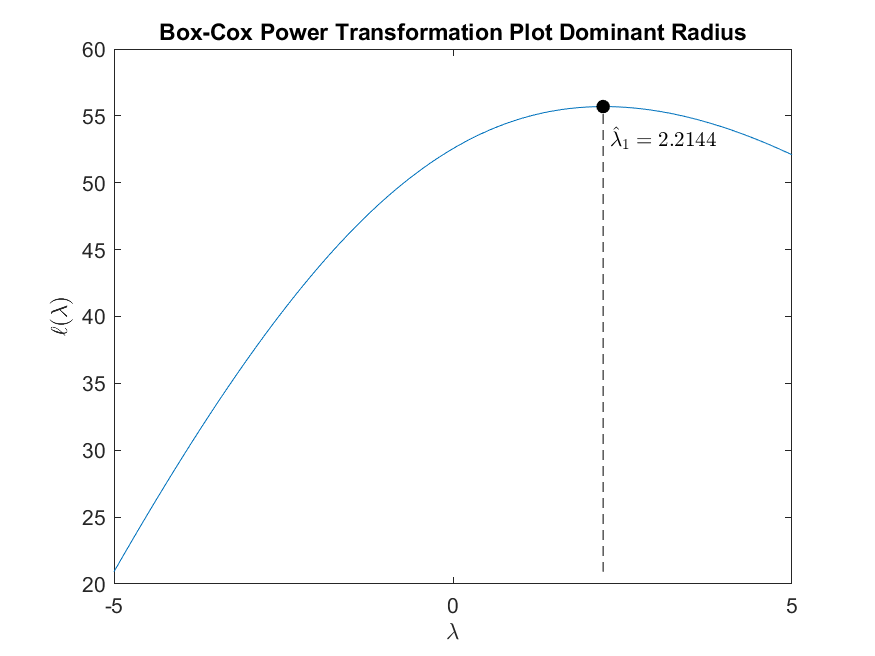
\includegraphics[scale=0.6]{./matlab/chapter-4/sol4.34.power.1.png}
    \end{figure}
\end{center}

\begin{center}
    \begin{figure}[H]
        \centering
        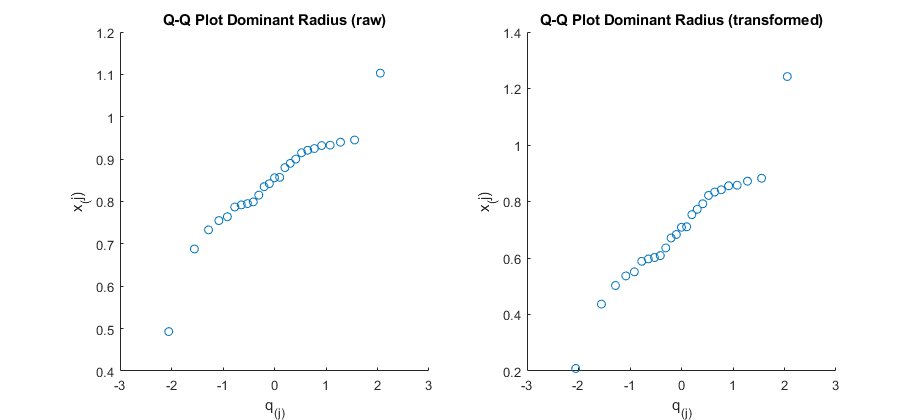
\includegraphics[scale=0.4]{./matlab/chapter-4/sol4.34.qq.1.png}
    \end{figure}
\end{center}

For ($x_{2}$), we're using the nondominant side of the radius bone found in the forearm to measure the mineral content via photon absorptiometry, and have 25 valid observations. The simulated 0.01, 0.05, and 0.10 level critical correlation coefficient test values for a sample size of 25 are, 0.9405, 0.9591, and 0.9665, respectively. The Q-Q correlation coefficient using the raw data was 0.9721, is larger than all three of these values, so the data would be considered normally distributed at the 0.01, 0.05, and 0.10 levels.

We don't really need to transform the data, but just to see how much better it can get, the Box-Cox power transformation max was 2.0942, so $x_{2}^{\prime} = x_{2}^{2.0942}$. The Q-Q correlation coefficient on the transformed data was 0.9804, so we do get some improvement. Below is the Q-Q plot for the raw data, which looks pretty good.

\begin{center}
    \begin{figure}[H]
        \centering
        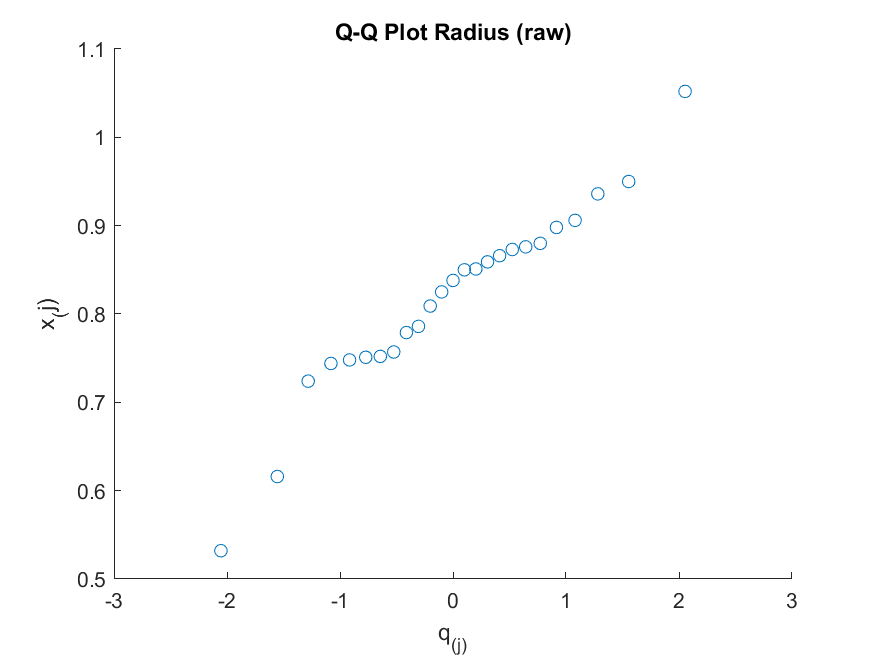
\includegraphics[scale=0.6]{./matlab/chapter-4/sol4.34.qq.2.png}
    \end{figure}
\end{center}

For ($x_{3}$), we're using the dominant side of the humerus bone found in the forearm to measure the mineral content via photon absorptiometry, and have 25 valid observations. The simulated 0.01, 0.05, and 0.10 level critical correlation coefficient test values for a sample size of 25 are, 0.9405, 0.9591, and 0.9665, respectively. The Q-Q correlation coefficient using the raw data was 0.9842, is larger than all three of these values, so the data would be considered normally distributed at the 0.01, 0.05, and 0.10 levels.

We don't really need to transform the data, but just to see how much better it can get, the Box-Cox power transformation max was 1.7535, so $x_{3}^{\prime} = x_{3}^{1.7535}$. The Q-Q correlation coefficient on the transformed data was 0.9903, so we do get a nice improvement. Below is the Q-Q plot for the raw data, which looks even better than the one for $x_{2}$.

\begin{center}
    \begin{figure}[H]
        \centering
        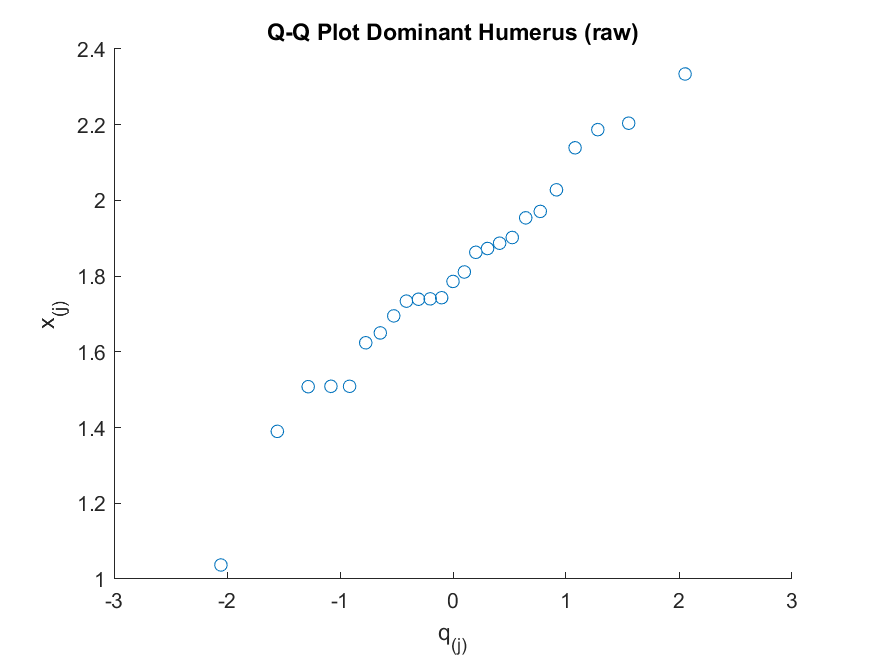
\includegraphics[scale=0.6]{./matlab/chapter-4/sol4.34.qq.3.png}
    \end{figure}
\end{center}

For ($x_{4}$), we're using the nondominant side of the humerus bone found in the forearm to measure the mineral content via photon absorptiometry, and have 25 valid observations. The simulated 0.01, 0.05, and 0.10 level critical correlation coefficient test values for a sample size of 25 are, 0.9405, 0.9591, and 0.9665, respectively. The Q-Q correlation coefficient using the raw data was 0.9901, is larger than all three of these values, so the data would be considered normally distributed at the 0.01, 0.05, and 0.10 levels.

We don't really need to transform the data, but just to see how much better it can get, the Box-Cox power transformation max was at 0.5711, so $x_{4}^{\prime} = x_{4}^{0.5711}$. The Q-Q correlation coefficient on the transformed data was 0.9907, so we do get a very slight improvement. Below is the Q-Q plot for the raw data, which looks nice and linear.

\begin{center}
    \begin{figure}[H]
        \centering
        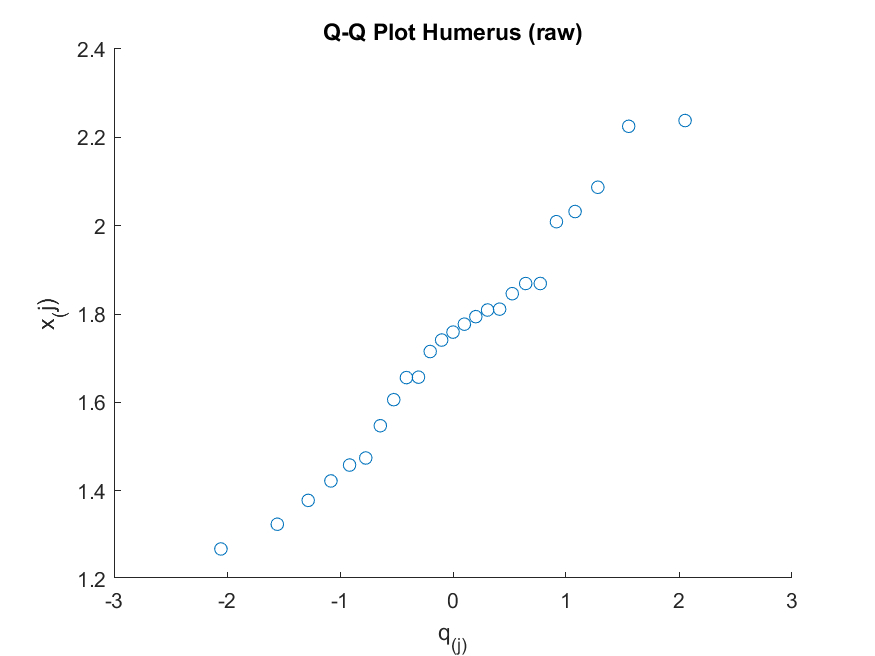
\includegraphics[scale=0.6]{./matlab/chapter-4/sol4.34.qq.4.png}
    \end{figure}
\end{center}

For ($x_{5}$), we're using the dominant side of the ulna bone found in the forearm to measure the mineral content via photon absorptiometry, and have 25 valid observations. The simulated 0.01, 0.05, and 0.10 level critical correlation coefficient test values for a sample size of 25 are, 0.9405, 0.9591, and 0.9665, respectively. The Q-Q correlation coefficient using the raw data was 0.9812, is larger than all three of these values, so the data would be considered normally distributed at the 0.01, 0.05, and 0.10 levels.

We don't really need to transform the data, but just to see how much better it can get, the Box-Cox power transformation max was at 0.8317 (close-ish to 1), so $x_{5}^{\prime} = x_{5}^{0.8317}$. The Q-Q correlation coefficient on the transformed data was 0.9811, so we do get a very slight improvement. Below is the Q-Q plot for the raw data, which looks good.

\begin{center}
    \begin{figure}[H]
        \centering
        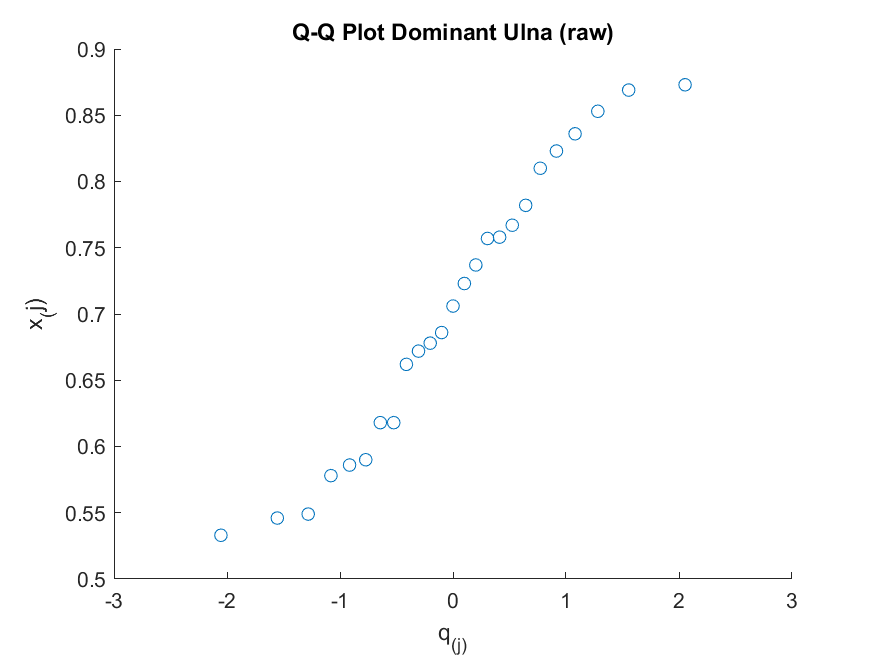
\includegraphics[scale=0.6]{./matlab/chapter-4/sol4.34.qq.5.png}
    \end{figure}
\end{center}

For ($x_{6}$), we're using the nondominant side of the ulna bone found in the forearm to measure the mineral content via photon absorptiometry, and have 25 valid observations. The simulated 0.01, 0.05, and 0.10 level critical correlation coefficient test values for a sample size of 25 are, 0.9405, 0.9591, and 0.9665, respectively. The Q-Q correlation coefficient using the raw data was 0.9940, is larger than all three of these values, so the data would be considered normally distributed at the 0.01, 0.05, and 0.10 levels.

We don't really need to transform the data, but just to see how much better it can get, the Box-Cox power transformation max was at 1.2926 (close-ish to 1), so $x_{6}^{\prime} = x_{6}^{1.2926}$. The Q-Q correlation coefficient on the transformed data was 0.9945, so we do get a very slight improvement. Below is the Q-Q plot for the raw data, which looks alright.

\begin{center}
    \begin{figure}[H]
        \centering
        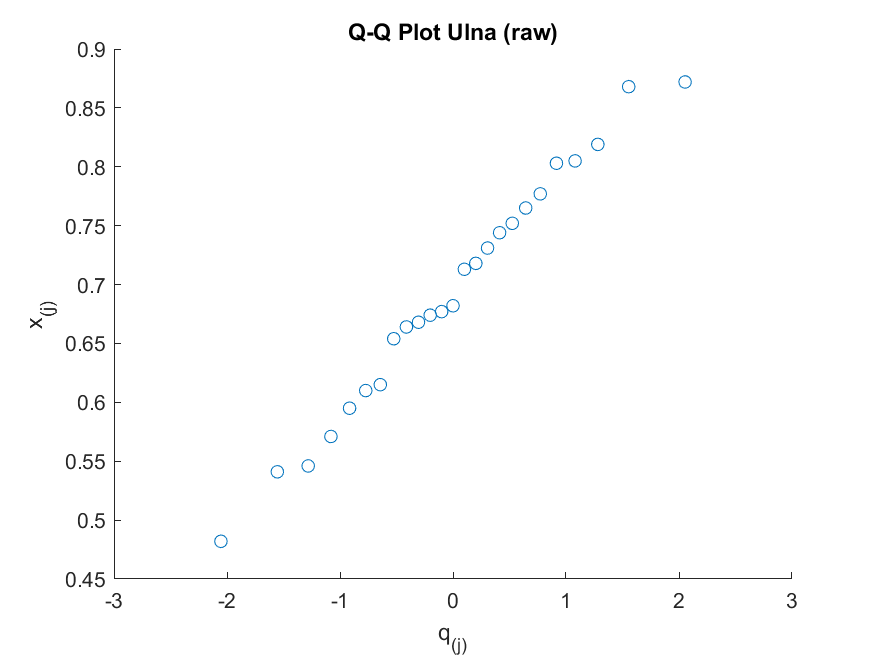
\includegraphics[scale=0.6]{./matlab/chapter-4/sol4.34.qq.6.png}
    \end{figure}
\end{center}

Checking out the bivariate, we have ${6 \choose 2} = 15$ pairs of variables to evaluate for

\[
\left\{
    \begin{NiceArray}{ccccc}
        (x_{1}, x_{2}), & (x_{1}, x_{3}), & (x_{1}, x_{4}), & (x_{1}, x_{5}), & (x_{1}, x_{6}), \\
        (x_{2}, x_{3}), & (x_{2}, x_{4}), & (x_{2}, x_{5}), & (x_{2}, x_{6}) & \\
        (x_{3}, x_{4}), & (x_{3}, x_{5}), & (x_{3}, x_{6}) & & \\
        (x_{4}, x_{5}), & (x_{4}, x_{6}), & & & \\
        (x_{5}, x_{6}) & & & & \\
    \end{NiceArray}
\right\}
\]

\begin{table}[H]
    \caption*{Proportion less than $\chi_{2}^{2}(0.50) = 1.3863$}
    \centering
    \begin{tabular}{lcc}
        \hline % chktex 44
        Variables & Raw Data & Transformed Data \\
        \hline % chktex 44
        $(x_{1}, x_{2})$ & 0.7200 &    0.6800 \\
        $(x_{1}, x_{3})$ & 0.6000 &    0.6000 \\
        $(x_{1}, x_{4})$ & 0.6000 &    0.5600 \\
        $(x_{1}, x_{5})$ & 0.6000 &    0.5200 \\
        $(x_{1}, x_{6})$ & 0.6000 &    0.6000 \\
        $(x_{2}, x_{3})$ & 0.7200 &    \textemdash~\\
        $(x_{2}, x_{4})$ & 0.5600 &    \textemdash~\\
        $(x_{2}, x_{5})$ & 0.5200 &    \textemdash~\\
        $(x_{2}, x_{6})$ & 0.6000 &    \textemdash~\\
        $(x_{3}, x_{4})$ & 0.5200 &    \textemdash~\\
        $(x_{3}, x_{5})$ & 0.4000 &    \textemdash~\\
        $(x_{3}, x_{6})$ & 0.5200 &    \textemdash~\\
        $(x_{4}, x_{5})$ & 0.4000 &    \textemdash~\\
        $(x_{4}, x_{6})$ & 0.4400 &    \textemdash~\\
        $(x_{5}, x_{7})$ & 0.4400 &    \textemdash~\\
        \hline % chktex 44
    \end{tabular}
\end{table}

I opted not to transform $x_{2}$ through $x_{6}$ and for the most part bivariate normality looks okay. The exceptions are $x_{1}$ and $x_{2}$, whose proportion of squared distance values less than 1.3862 is 72\% for raw data and 68\% for transformed $x_{1}$, when we'd expect to see 50\%. Also, $x_{2}$ and $x_{3}$ has a percentage of 73\%. It might be worth it to transform $x_{2}$.